\subsection{Definition of summable families of measures}

Let \((\lambda_{\alpha})_{\alpha \in \mathrm{A}}\) be a family of positive measures on a locally compact space \(X\) ; the family \((\lambda_{\alpha})_{\alpha \in \mathrm{A}}\) is said to be a summable family of measures if it is summable in the vector space \(\mathcal{M}(X)\) of real measures on \(X\) , equipped with the vague topology (GT, III, §5, No.~1). This amounts to saying that for every function \(f \in \mathcal{H}(X)\) , the family of numbers \(\lambda_{\alpha}(f)\) is summable in \(\mathbf{R}\) . For, this condition is obviously necessary; conversely, if it is satisfied then the linear form \(f \mapsto \sum_{\alpha \in \mathrm{A}} \lambda_{\alpha}(f)\) on \(\mathcal{H}(X)\) is positive, hence is a positive measure \(\nu\) (Ch. III, §1, No.~5, Th. 1), and one verifies immediately that the finite partial sums of the family \((\lambda_{\alpha})\) converge vaguely to \(\nu\) , with respect to the section filter of the set of finite subsets of \(A\) (GT, III, §5, No.~1, Def. 1).

Since every element of \(\mathcal{H}(\mathrm{X})\) is the difference of two elements of \(\mathcal{H}_{+}(\mathrm{X})\) , the family \((\lambda_{\alpha})\) is summable if and only if

\[
\sum_ {\alpha \in A} \lambda_ {\alpha} (f) <   + \infty\tag{1}
\]

for every function \(f \in \mathcal{K}_{+}(X)\) . This condition is also equivalent to the following:

\[
\sum_ {\alpha \in \mathrm{A}} \lambda_ {\alpha} (\mathrm{K}) <   + \infty\tag{2}
\]

for every compact set \(\mathrm{K} \subset \mathrm{X}\) .

For, (2) implies (1) because \(f \leqslant \|f\| \cdot \varphi_{\mathrm{S}}\) , where S denotes the compact support of \(f\) . Conversely, if K is a compact set, there exists a function \(f \in \mathcal{K}_{+}(\mathbf{X})\) such that \(\varphi_{\mathrm{K}} \leqslant f\) (Ch. III, §1, No.~2, Lemma 1), and it follows that (1) implies (2).

Remarks. --- 1) It is immediate that, when the family \((\lambda_{\alpha})_{\alpha \in A}\) is summable, its sum is the supremum in \(\mathcal{M}_{+}(X)\) of the finite partial sums \(\sum_{\alpha \in J} \lambda_{\alpha}\) , where \(J\) runs over the set of finite subsets of \(A\) .

\pandocbounded{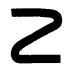
\includegraphics[keepaspectratio]{images/part002_9de8d58d.jpg}}

\begin{enumerate}
\def\labelenumi{\arabic{enumi})}
\setcounter{enumi}{1}
\tightlist
\item
  Let \((\theta_{\alpha})_{\alpha\in\mathbb{A}}\) be a family of complex measures on X; the family \((\theta_{\alpha})\) is said to be summable if the family \((|\theta_{\alpha}|)\) of positive measures is summable; it is not sufficient for this that the family \((\theta_{\alpha})\) be summable in the vector space \(\mathcal{M}(X;\mathbf{C})\) equipped with the vague topology (cf.~Exer. 3).
\end{enumerate}

